% !TeX root = ../main.tex

\chapter{基于3D高斯泼溅的水下三维重建}
3D 高斯泼溅(3DGS)\cite{3DGS} 已逐步取代神经辐射场(NeRF)\cite{nerf} 技术,成为场景重建领域的热门工具。
3DGS 通过其独特的高斯表示方法,能够在复杂的三维环境中提供更为精确的场景重建能力。与传统的 NeRF 方法相比,3DGS 在处理动态场景时表现出更高的灵活性和适应性。
然而,目前尚缺乏针对水下环境的充分验证与应用研究,主要原因在于缺少专门用于此类任务的水下场景数据集支持。
此外,水下图像存在固有的退化效应(如光散射、色偏)及水流造成的动态扰动,对水下三位重建任务的鲁棒性提出了更高的要求。
图像退化问题可以通过前一章中提出的图像恢复算法进行原始采集图像的质量增强,从而缓解劣质图形在三维重建时对相机位姿估计、点云生成等数据预处理的影响。
但是水下场景中存在的水流造成的动态扰动,需要一种能够有效抑制动态干扰的重建方法。
得益于神经网络的时空预测能力,3DGS 在动态场景的重建中也具备高质量的场景复现能力,
为此,本章提出了一种基于 3DGS 和 KAN \cite{kan}变形机制的水下场景感知增强框架。
该框架旨在通过多阶段的训练模式寻找出特定时刻下的静态场景表示,从而抑制运动干扰并且保留水下场景的基础静态特征。
同时,本章构建了一个专门面向水下场景重建的数据集,并在此数据集上对方法有效性进行验证。
实验结果表明,与其他基准方法相比,本章提出的框架在水下动态场景重建的准确性和鲁棒性方面具有显著优势。

\section{水下动态场景的3D高斯泼溅方法} \label{sec:4dgs}
由于水流造成的动态扰动,场景中的同一物体在不同时间的多帧图像中会表现不同的外观特征以及位置,这会导致重建结果中出现模糊和重影现象。
3D 高斯泼溅方法可以直接对场景信息进行显式表示,这为动态场景建模提供了一种灵活的解决方案,
其核心思想是通过变形每个时间点的 3D 高斯表示,寻找符合动态场景重建的最优变形方法。
通过这种方法,可以在动态场景中更好地捕捉物体的运动轨迹和形变特征。
目前,利用神经网络学习位置与时间信息的映射关系已成为主流方案。
在此基础上,本章重新设计了基于时空信息编码与特征解码的4D高斯泼溅\cite{4DGS}框架,
如图\ref{img:4dgs}所示,该框架通过时空结构编码器高效提取 3D 高斯的时空特征,并结合特征解码器实现高斯变形预测,从而完成水下动态场景的重建,
能够在动态场景中实现高精度的重建效果,尤其是在处理复杂的水下环境时,能够有效应对光线变化和水流扰动带来的挑战。
\begin{figure}[ht]
    \centering
    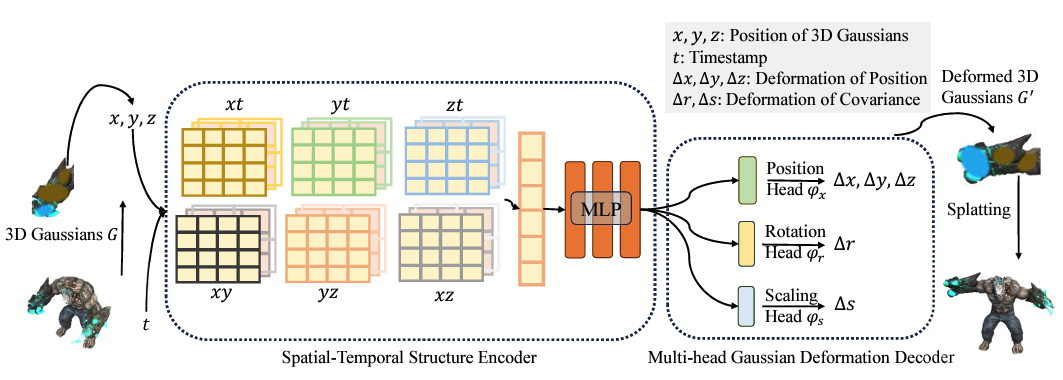
\includegraphics[width=0.99\textwidth]{figures/ch4/4dgs.pdf}
    \vspace{4mm}
    \caption{基于 3D 高斯泼溅的水下动态场景重建框架}
    \label{img:4dgs}
    \vspace{4mm}
\end{figure}

\subsection{3D高斯时空编码器}
对于一个大小为$H, W, L$的三维网格空间来说,其空间复杂度呈正相关关系。
较高的空间分辨率可以保证最终重建结果的细节质量,但会导致该时空网格的内存占用无法承受。
为了解决这个问题,本章提出了一种基于HexPlane\cite{hex_plane}的时空结构编码器,可以有效减少空间网格的内存占用,避免维度爆炸。

动态场景中的相邻 3D 高斯通常具有显著的时空信息相似性,
特别是在受到单一方向的水流扰动时,这些相邻 3D 高斯在时间维度上表现出的相似性特征尤为明显。
HexPlane 模块可以有效利用这种相邻时空信息的相似性质,对高维时空信息进行特征分解,从而优化内存占用并降低计算复杂度。
基于 HexPlane 特征分解模块,本章设计了一种高效的时空结构编码器 $\mathcal{H}$,
该编码器由多个分辨率的二维空间网格特征和一个多层感知机(MLP)模块组成。
其主要目标是结合 3D 高斯的位置与时间信息,将其映射到低维特征空间,为后续多头解码器进行变形预测提供支持。

为了避免高维空间的维度灾难,本章的HexPlane特征分解采用了K-Planes\cite{k-planes}的方法将每个点的特征分解为它在空间中的特征和它在每个轴(XYZ)上关于时间的特征,从而优化内存占用并降低计算复杂度。
具体做法是将原始 4D 神经体素分解为 6 个独立的平面模块,这些模块能够有效表示一定区域内的 3D 高斯,并通过时间维度进一步捕捉高斯变形信息。
因此3D时空结构编码器$\mathcal{H}$包含6个多分辨率平面模块$R_l(i,j)$和一个小型MLP模块$\phi_d$,如公式\ref{eq:encoder_H}所示:
\begin{equation}
\label{eq:encoder_H}
\mathcal{H}(G, t) = \{ R_l(i,j), \phi_d \ | \ (i,j) \in \{(x,y), (x,z), (y,z), (x,t), (y,t), (z,t)\}, l \in \{1, 2\} \}
\end{equation}

其中,$\mathcal{X} = (x, y, z)$表示3D高斯的中心位置,$l$表示上采样的尺度,
$R(i,j)$是每个体素平面模块,维度为$R(i,j) \in \mathbb{R}^{h \times l N_i \times l N_j}$,
其中$h$表示平面中单个网格特征的维度,$N_i,N_j$表示每个平面体素网格的基本分辨率。

为提取每个体素特征,需要在6个2D体素平面中对3D高斯体的信息进行编码,可以使用双线性插值的方法查询平面体素网格四个顶点的特征,计算公式为:
\begin{equation}
f_h = \bigcup_l \prod \text{interp}(R_l(i,j)), \quad (i,j) \in \{(x,y),(x,z),(y,z),(x,t),(y,t),(z,t)\}
\end{equation}

其中,$f_h \in \mathbb{R}^{h \times l}$表示神经体素的特征。
随后,MLP 模块 $\phi_d$ 融合所有特征以生成最终的编码表示:
\begin{equation}
f_d = \phi_d(f_h)
\end{equation}  

该编码过程不仅可以高效捕获动态场景中时空特征的变化,还为后续高斯变形计算奠定基础,在动态场景中更好地捕捉物体的运动轨迹和形变特征,提高重建的精度和稳定性

\subsection{基于KAN的特征解码器}
时空结构编码器生成的 3D 高斯特征随后被输入到多头高斯变形解码器 $\mathcal{D}$ 中,以计算每个 3D 高斯在不同时刻下的变形信息。
该解码器包含多个KAN模块,分别用于估计位置变形$\Delta \mathcal{X}$、旋转变形$\Delta r$和缩放变形$\Delta s$。
这些变形信息构成了变形后的 3D 高斯表示$G^\prime=\{\mathcal{X}^\prime, s^\prime, r^\prime, \sigma, \mathcal{C} \}$。
KAN 模块通过学习神经元的最优激活方式,在保证解码准确性的同时减少了所需的神经元数量。
基于KAN的特征解码器通过自适应的方式预测形变量,最终的变形3D高斯可以表示为:
\begin{equation}
    G^\prime = \{ \mathcal{X} + \Delta \mathcal{X}, r + \Delta r, s + \Delta s, \alpha + \Delta \alpha, \mathcal{C} + \Delta \mathcal{C} \}
\end{equation}

不同时刻下的3D高斯可以有效处理水下环境中的动态特征,生成精准的动态场景重建结果。

\section{水下静态三维场景自对抗训练}
\subsection{多阶段训练模式}
在水下复杂环境中,水流引发的动态干扰会导致场景中物体晃动,使得完全静态的水下场景重建变得极具挑战性。
尽管基于动态场景重建的方法能够在一定程度上保留动态效果并生成高质量、逼真的新视图,
但在单目相机拍摄的水下动态场景中,某些时刻可能出现异常的重建现象。这种现象通常由以下原因导致:
(1)某些时刻运动干扰过于强烈,画面质量显著下降;
(2)动态场景数据集中缺乏足够的视角覆盖,导致 3D 高斯变形预测出现误差。

真实世界中水下重建场景的对象位置相对固定,且水流带来的扰动具有一定周期性,导致不同视角下的场景存在相似的高频信息。
为捕捉这些高频静态特征并实现高质量水下场景重建,本章提出了一种带有场景过滤模块的多阶段训练模式。
如图 \ref{img:3_stage} 所示,该模式分为以下三个阶段:初始化训练阶段、动态场景训练阶段和目标场景训练阶段。
\begin{figure}[htbp]
    \centering
    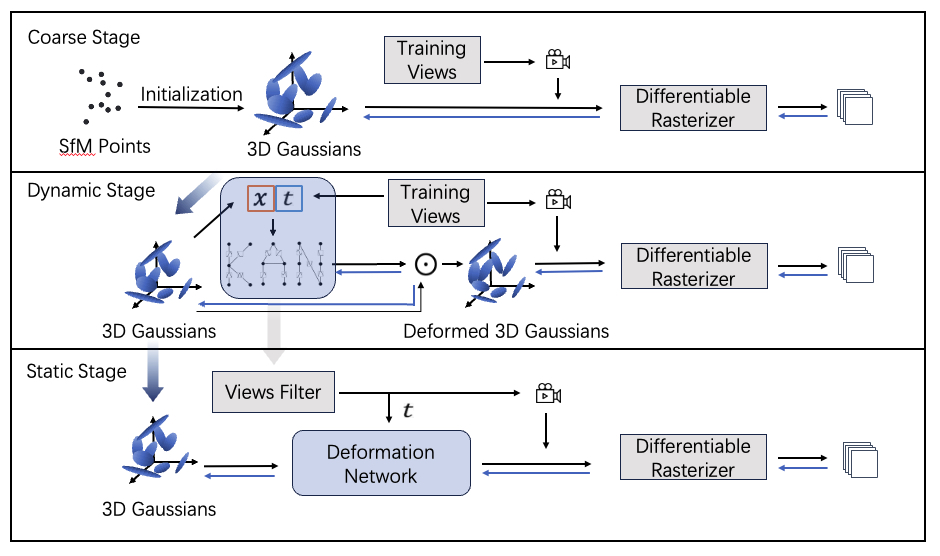
\includegraphics[width=0.95\textwidth]{figures/ch4/3_stage.pdf}
    \caption{多阶段训练模式}
    \label{img:3_stage}
\end{figure}

(1)初始化训练阶段:利用基于结构化运动(SfM)方法\cite{sfm1}\cite{sfm2}初始化的点云,对 3D 高斯初始表示进行优化。
\begin{equation}
    G_1 = Train_{w/o-\mathcal{F} }(\mathcal{C})
\end{equation}
其中,$G_1$为初始化训练的3D高斯,$\mathcal{C}$为完整的训练相机序列数据,$\mathcal{F}$为基于3D高斯时空编码器与KAN的特征解码器网络。
该阶段旨在快速完成初步重建,缓解动态重建初期的不稳定性,避免后续训练阶段中由于梯度爆炸出现程序崩溃,故暂时不使用变形预测网络$\mathcal{F}$。

(2)动态场景训练阶段:通过章节 \ref{sec:4dgs} 中介绍的 3D 高斯时空编码器与基于 KAN 的特征解码器构成的变形预测网络$\mathcal{F}$进行动态场景的训练,从而提高水下动态重建质量,同时保留动态效果。
\begin{equation}
    G_2, \mathcal{F} = Train_{w/-\mathcal{F} }(\mathcal{C})
\end{equation}
其中,$G_2$为动态场景训练的 3D 初始化高斯,按照$\mathcal{C}$中的不同相机位姿的时间和变相预测网络$\mathcal{F}$对$G_2$的3D高斯进行变形预测,
对变形后的 3D 高斯$G_2^\prime$进行光栅化渲染,利用梯度传播同时优化$G_2$和$\mathcal{F}$。

(3)目标场景训练阶段:首先结合上一阶段优化的变形预测网络$\mathcal{F}$和$G_2$对完整的训练数据$\mathcal{C}$进行筛选,
提取其中的最高频出现的静态场景数据$\mathcal{C}_s$:
\begin{equation}
    \mathcal{C}_s = Filter(G_2, \mathcal{C}, \mathcal{F})
\end{equation}
最后按照新的训练数据$\mathcal{C}_s$进行目标场景训练,从而实现目标静态场景的高质量重建,同时依旧保留 3D 高斯变形机制,以提高重建的鲁棒性。
\begin{equation}
    G_3, \mathcal{F} = Train_{w/-\mathcal{F} }(\mathcal{C}_s)
\end{equation}

通过采用这种多阶段训练模式,利用筛选后的训练数据$\mathcal{C}_s$去除原始数据中的干扰数据,进一步提升了静态场景的重建精度和稳定性。

\subsection{场景过滤模块}
为确保在目标水下静态场景训练阶段能够高效筛选出静态优质片段,本章设计了一种基于时序分析的自适应场景过滤模块。
该模块通过分析场景中3D高斯的时序变化特征,结合多尺度静态片段融合策略,实现了对水下场景静态片段数据的精确提取。
如图\ref{img:filter}所示,该模块包含时序差分分析、自适应阈值分割和多尺度静态片段融合三个关键步骤。
\begin{figure}[htbp]
    \centering
    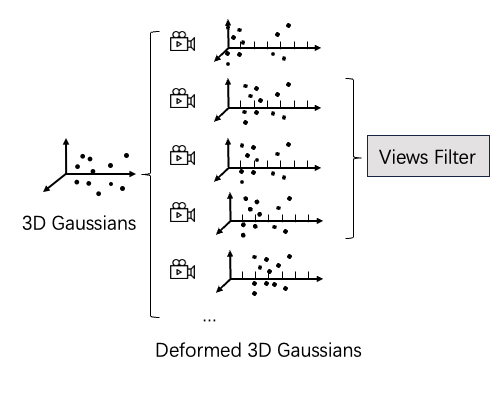
\includegraphics[width=0.95\textwidth]{figures/ch4/filter.pdf}
    \caption{场景过滤模块}
    \label{img:filter}
\end{figure}

\subsubsection{时序差分分析}
基于4.2.1节中第二阶段训练的3D高斯变形预测网络$\mathcal{F}$,可以得到所有训练数据相机序列$\mathcal{C}$对应时刻$t$下3D高斯位置变形$\mathcal{X}_t=\mathcal{F}(G, t)$,其中$G$为上阶段训练的初始化3D高斯。
接下来对相邻时刻的3D高斯变形进行差分分析,计算每个时间步的场景变化量$\delta_i$。
例如,对于时刻$t_i$和$t_{i+1}$,通过计算变形后高斯位置$\mathcal{X}_i$和$\mathcal{X}_{i+1}$之间的欧氏距离来量化场景变化:
\begin{equation}
\delta_i = \|\mathcal{X}_{i+1} - \mathcal{X}_i\|_2
\end{equation}
统计所有相邻时刻的场景变化量得到时序差分序列$\delta$。

为减少噪声影响,对时序数据采用滑动窗口平滑处理得到的时序差分序列$\delta_s$。
具体做法是,对于每个时刻$i$,通过在其前后$\lfloor\omega/2\rfloor$个时刻范围内计算均值来平滑当前时刻的变化量:

\begin{equation}
\delta_s^i = \frac{1}{w_{\text{end}} - w_{\text{start}} + 1} \sum_{j=w_{\text{start}}}^{w_{\text{end}}} \delta_j
\end{equation}

其中,$w_{\text{start}} = \max(1, i - \lfloor\omega/2\rfloor)$和$w_{\text{end}} = \min(|\Delta|, i + \lfloor\omega/2\rfloor)$分别表示滑动窗口的起始和结束位置。
这种自适应窗口边界的处理方式确保了序列首尾处的平滑操作也能得到合理的结果。最终得到平滑后的时序差分序列$\delta_s$。

窗口大小$\omega$的选择需要在平滑效果和时间分辨率之间进行权衡。
较大的窗口尺寸可以更好地抑制噪声,但可能会模糊时间边界,导致相邻静态片段之间的过渡不够清晰;
较小的窗口尺寸能够保持较高的时间分辨率,有利于准确定位场景变化的时间点,但可能会收到本身数据质量的影响。
本章采用窗口大小为5的滑动窗口进行时序差分分析,
该窗口大小能有效平滑数据之间的短期变化,为后续的静态片段提取提供了可靠的基础。

\subsubsection{自适应阈值分割}
本模块采用OTSU自适应阈值算法对平滑后的时序差分序列进行分割。
该算法通过最大化类间方差的方式,自动确定最优分割阈值$\tau_{\text{otsu}}$,常常在图像分割任务中用于分割出前景和背景。具体计算步骤如下:

(1)首先统计出序列$\delta_s$的直方图分布$\mathcal{H}$,将数据范围等分为50个区间,计算每个区间的中心值$x_i$和对应的频数$n_i$;

(2)计算序列的总样本数$N$和全局均值$\mu_T$:
\begin{equation}
N = \sum_{i=1}^{50} n_i, \quad \mu_T = \frac{1}{N}\sum_{i=1}^{50} x_i \cdot n_i
\end{equation}

(3)对每个可能的阈值$\tau$,计算前景类(小于等于阈值)的累积统计量:
\begin{equation}
n_b(\tau) = \sum_{i=1}^{\tau} n_i, \quad \mu_b(\tau) = \sum_{i=1}^{\tau} x_i \cdot n_i
\end{equation}

(4)计算前景类和背景类的类间方差:
\begin{equation}
\sigma_B^2(\tau) = \frac{n_b(\tau)}{N} \cdot \frac{N-n_b(\tau)}{N} \cdot [\frac{\mu_b(\tau)}{n_b(\tau)} - \frac{\mu_T \cdot N-\mu_b(\tau)}{N-n_b(\tau)}]^2
\end{equation}

(5)选择使类间方差最大的阈值作为最优分割阈值:
\begin{equation}
\tau_{\text{otsu}} = \arg\max_{\tau} \{\sigma_B^2(\tau)\}
\end{equation}

这种基于类间方差最大化的阈值选择方法,能够自动找到最优的分割点,将时序差分序列$\delta_s$分为多个静态片段(低于阈值)$\mathcal{S}$和动态片段(高于阈值)两类。

OTSU算法的优势在于其自适应性,无需人工设定固定阈值,能够根据场景的实际变化特征自动调整分割阈值,提高了方法的泛化能力。

\subsubsection{多尺度静态片段融合}
在得到多个静态片段后,还需要对这些片段进行相似性检查,以确保最终的静态片段集合$\mathcal{S}$中只包含具有相似静态场景特征的片段。
该策略不仅考虑了单个静态片段的时间连续性,还通过跨片段的相似性分析,
实现了对具有相似静态特征但在时间上不连续的片段的有效融合:

(1) 首先识别最长的静态片段$\mathcal{S}_{\text{max}}$,并从中随机采样参考数据$\mathcal{R}$。
   最长静态片段通常包含了场景最稳定的部分,因此其特征可以作为评估其他片段的可靠基准;

(2)对其他静态片段$s\in\mathcal{S}$进行验证,计算其采样数据$\mathcal{D}_s$与参考数据$\mathcal{R}$的相似度:
\begin{equation}
\text{sim}(\mathcal{D}_s, \mathcal{R}) = \frac{1}{|\mathcal{D}_s||\mathcal{R}|}\sum_{d \in \mathcal{D}_s}\sum_{r \in \mathcal{R}}\|d - r\|_2
\end{equation}

(3)当相似度满足阈值条件时,将该静态片段加入有效片段集合$\mathcal{S}_{\text{valid}}$:
\begin{equation}
\mathcal{S}_{\text{valid}} = \{s \ | \ \text{sim}(\mathcal{D}_s, \mathcal{R}) < \tau_{\text{otsu}}\}
\end{equation}

最终,通过合并所有有效静态片段,得到用于静态场景重建的相机序列$\mathcal{C}_s=\bigcup_{s\in\mathcal{S}_{\text{valid}}}\mathcal{D}_s$。
该多尺度融合策略不仅保证了静态特征提取的准确性,还提高了算法对水下场景周期性运动的适应能力。
特别地,通过随机采样和相似度比较的方式,该策略能够有效处理由于水流扰动导致的周期性运动,
在保留场景静态结构的同时,避免了过度筛选导致的信息丢失。

\subsection{损失函数设计}
与其他重建方法类似\cite{3DGS}\cite{tineuvox}\cite{dnerf},本文采用L1颜色损失(L1 Color Loss)来监督训练过程,
确保生成的3D高斯在颜色方面与目标场景的实际颜色保持一致。
此外,还引入了基于网格的全变差损失(Total Variation Loss,$\mathcal{L}_{tv}$),
以减少噪声并提高重建结果的平滑性。

L1颜色损失用于衡量生成的场景颜色与真实场景颜色之间的绝对误差,计算公式为:
\begin{equation}
    \mathcal{L}_{color} = \sum_{i} \left\| \hat{C}_i - C_i \right\|_1
\end{equation}

其中,$\hat{C}_i$是模型生成的第$i$个像素的颜色值,$C_i$是对应的真实颜色值。

全变差损失通过度量网格中像素值的梯度变化来减少不必要的细节和噪声,从而增强重建结果的平滑性和稳定性,特别是在处理高频细节和复杂动态场景时。
其计算公式为:
\begin{equation}
    \mathcal{L}_{tv} = \sum_{i,j} \left\| \nabla G(i,j) \right\|_2
\end{equation}

其中,$\nabla G(i,j)$表示网格中位置$(i,j)$的梯度,衡量的是相邻体素之间的变化。这个损失项在训练过程中有助于避免模型过度拟合细节,从而提高重建的鲁棒性。

最终的总损失函数 $\mathcal{L}_{total}$ 结合了上述两种损失,通过加权组合实现颜色一致性与平滑性的平衡:
$$
\mathcal{L}_{total} = \mathcal{L}_{color} + \lambda_{tv} \cdot \mathcal{L}_{tv}
$$

其中,$\lambda_{tv}$是全变差损失的权重系数,用于平衡颜色损失和平滑性损失之间的影响。
通过最小化总损失函数,模型不仅能够实现对动态场景的高精度重建,还能有效抑制噪声的干扰,保证生成结果的平滑性和视觉质量。

\section{实验结果}
\subsection{水下重建数据集}
为验证水下重建方法的有效性,本章制作了一个专用水下重建数据集 3DUW。
首先,搭建了一个可控的人造水下场景,并通过组合不同的环境条件(水流扰动和色偏)生成四组配对数据集,以测试算法在动态扰动抑制和颜色校正(去色偏)能力上的表现。
如图 \ref{img:3DUW} 所示,不同环境条件下的数据集为算法的泛化性能验证提供了丰富的场景样本。
随后,使用单目相机从多个角度和时间点采集水下场景图像,应用SfM算法\cite{sfm1}\cite{sfm2}对数据进行预处理,生成每张图像对应的相机位姿信息和初始点云。
\begin{figure}
    \centering
    \includegraphics[width=0.95\textwidth]{figures/ch4/3DUW.pdf}
    \caption{3DUW 数据集}
    \label{img:3DUW}
\end{figure}

另外,由于3DGS的重建质量在很大程度上依赖于SfM中获得的初始点云。
而水下原始图像由于存在不同程度的模糊和色偏,导致SfM算法难以提取准确的特征点,只会产生稀疏的点云。
为了形成一个更加密集的点云,在获取水下图像后,使用K-Nearest-Neighbor(KNN)算法在现有点的外围添加额外的点。
算法\ref{eq:knn}描述了向原有稀疏点云添加补充点的过程。
\begin{algorithm}[t]
    \caption{\label{eq:knn}添加额外点云}
    \KwIn{$\mathcal{G}$: 从 SfM 计算的点云}
    \KwIn{$K$: 需要查找的邻近点个数}
    \KwIn{$N_p$: 需要生成的额外点个数}
    \KwIn{$t_d$: 新生成点与已有点之间的最小距离要求}
    
    $P_\text{add} \leftarrow \text{GenerateRandomPoints}(\mathcal{P}, N_p)$\tcp*{均匀采样生成 $N_p$ 个新点}
    
    \For{每个 $p \in P_\text{add}$}{
        $\mathcal{P}_\text{knn} \leftarrow \text{FindNearestNeighbors}(\mathcal{P}, p, K)$\tcp*{找到 $p$ 在 $\mathcal{P}$ 中的 $K$ 个最近邻点}
        $\mathcal{P}_\text{valid} \leftarrow \text{CheckDistance}(\mathcal{P}_\text{knn}, p, t_d)$\tcp*{筛选出与 $p$ 距离满足要求的邻居点}
    
        \If{$|\mathcal{P}_\text{valid}| > 0$}{
            $p_c \leftarrow \text{LinearInterpolate}(\mathcal{P}_\text{valid}, p)$\tcp*{线性插值生成新点的颜色}
            $\text{AddToPointCloud}(\mathcal{P}, p, p_c)$\tcp*{将新点添加到点云 $\mathcal{P}$ 中}
        }
    }
\end{algorithm}

首先,通过均匀采样的方法在点云范围内生成$N_p$个随机的新点$P_\text{add}$。对于每个新点$p$,算法利用KNN方法从初始点云中找到其K个最近邻点,构成候选邻域集合$\mathcal{P}_\text{knn}$。
随后,通过检查邻近点与新点之间的距离,通过$t_d$筛选出满足最小距离要求的有效邻居点集合$\mathcal{P}_\text{valid}$。
如果有效邻居点集合非空,算法通过对有效邻居点的颜色信息进行线性插值,估算新点的颜色属性,并将该点及其颜色属性添加到点云中,完成补充点的生成。
这样的操作确保了新增点既满足稠密性需求,又与原始点云保持一致的几何和颜色特性。
该算法通过逐点更新的方式动态扩展了点云密度,同时有效避免了新增点与原始点过度重叠或无效分布的问题,为水下重建提供了更加丰富且高质量的点云数据支撑。

\subsection{实验设置}
为验证本章提出水下三维重建方法的性能和鲁棒性,实验选用了两组真实水下重建数据集:自制的 3DUW 数据集和公开数据集 SeaThru-NeRF\cite{seathru}。
其中3DUW为自制数据集,SeaThru-NeRF包含了三个不同的海洋中潜水获得的多图像水下场景:
以色列埃拉特的红海海域(SeaThru-NeRF-1,29张)、加勒比海库拉索海域(SeaThru-NeRF-2,21张)和太平洋巴拿马运河水域(SeaThru-NeRF-3,18张)。

两组数据集的划分如表 \ref{tab:recondata_split} 所示。
\begin{table}[htbp]
    \centering
    \caption{水下重建数据集划分}
    \label{tab:recondata_split}
    \begin{tabular}{cccc}
        \toprule
        数据集 & 训练集 & 测试集 & 共计 \\
        \midrule
        3DUW-1 & 100 & 50 & 150 \\
        3DUW-2 & 100 & 50 & 150 \\
        3DUW-3 & 100 & 50 & 150 \\
        3DUW-4 & 100 & 50 & 150 \\
        SeaThru-NeRF-1 & 22 & 7 & 29 \\
        SeaThru-NeRF-2 & 15 & 6 & 21 \\
        SeaThru-NeRF-3 & 15 & 3 & 18 \\
        \bottomrule
    \end{tabular}
\end{table}
实验的时空编码器与解码器均基于 PyTorch 框架\cite{pytorch}实现,利用其高效的深度学习工具链保证了模型的开发与训练效率。
所有实验均在单张 RTX 3060 GPU 上完成,批量大小为1,初始化训练、动态场景训练和目标场景训练的迭代次数分别设置为 3000 次、20000 次和 10000 次。

\subsection{定量评价}
为全面评估水下场景重建方法的性能,实验采用除章节\ref{sec:quantitative}中的参考指标PSNR与SSIM外,还引入了感知质量指标以及渲染时的运行帧率。

(1)感知质量指标(LPIPS)\cite{lpips}: 人类可以快速评估两幅图像之间的感知相似性,但是其背后的底层过程非常复杂,涉及对图像不同尺度的特征的比较过程。
因此,LPIPS 提出了使用预训练的深度网络来提取图像特征,然后计算这些特征之间的距离,以评估图像之间的感知相似度;
\begin{equation}
    d(x, x_0) = \sum_{l} \frac{1}{H_l W_l} \sum_{h,w} \left\| w_l \odot (\hat{y}^l_{hw} - \hat{y}^l_{0hw}) \right\|_2^2
\end{equation}

其中,$x$和$x_0$分别表示重建图像和参考图像,$H_l,W_l$表示图像在第$l$个尺度上的特征图的尺寸,$\hat{y}^l_{hw}$和$\hat{y}^l_{0hw}$表示图像在该尺度上的特征图在位置$(h, w)$的值,$w_l$是第$l$个尺度的权重系数。

(2)运行帧率(FPS):使用模型在1s内可以光栅化渲染的图像数量,衡量模型的重建时运行速度。

实验对包括 TiNeuVox\cite{tineuvox}、3DGS\cite{3DGS}、4DGS\cite{4DGS}和 Sea-NeRF\cite{seathru}
在内的多个基线方法进行了比较,实验结果见表 \ref{tab:res_3duw}和\ref{tab:res_seanerf},
由于本章提出的方法会对原始训练数据进行筛选,因此,测试集上的实验仅比较场景过滤模块筛选后的数据,以确保评价的公平性和一致性。

\begin{table} [htbp]
    \small
    \centering
    \caption{不同方法在数据集 3DUW 上的定量结果。}
    \setlength{\tabcolsep}{10pt}
    \begin{tabular}{lcccccc} 
    \toprule
    Model  & PSNR(dB)↑ & SSIM↑ & LPIPS↓ & Time↓ &  FPS ↑  \\
    \midrule  
    Sea-NeRF\cite{seathru} & 21.09& 0.92 & 0.09 & 55 mins & 1.59\\
    3DGS~\cite{3DGS} &22.34 & 0.91 & 0.08 & \textcolor{red}{\textbf{14}} mins  & \textcolor{red}{\textbf{94}}\\
    TiNeuVox~\cite{tineuvox}  & 28.81 & 0.95 &  0.03 & 60 mins & 0.79\\ 
    4DGS\cite{4DGS} & 34.22&\textcolor{red}{\textbf{0.98}} &\textcolor{red}{\textbf{0.02}}& 27 mins&44 \\
    Ours & \textcolor{red}{\textbf{34.58}} & \textcolor{red}{\textbf{0.98}} & \textcolor{red}{\textbf{0.02}} & 38 mins & \textcolor{red}{\textbf{94}}\\
    \bottomrule
    \end{tabular}  
    \label{tab:res_3duw}
\end{table}
    
\begin{table} [htbp]
    \small
    \centering
    \caption{不同方法在数据集 SeaThru-NeRF 上的定量结果。}
    \setlength{\tabcolsep}{10pt}
    \begin{tabular}{lcccccc} 
    \toprule
    Model  & PSNR(dB)↑ & SSIM↑ & LPIPS↓ & Time↓ &  FPS ↑  \\ 
    \midrule  
    Sea-NeRF\cite{seathru} & 32.79 & 0.97 & 0.03 & 53 mins & 1.64\\
    3DGS~\cite{3DGS} &32.84 & 0.93 & 0.08&\textcolor{red}{\textbf{13}} mins  &\textcolor{red}{\textbf{94}}\\
    TiNeuVox~\cite{tineuvox}  & 32.67 & 0.97 &  0.04 & 61 mins & 0.79\\ 
    4DGS\cite{4DGS} & 32.05&\textcolor{red}{\textbf{0.98}} &\textcolor{red}{\textbf{0.02}}& 27 mins&42 \\
    Ours & \textcolor{red}{\textbf{32.90}} & \textcolor{red}{\textbf{0.98}} & \textcolor{red}{\textbf{0.02}} & 40 mins & \textcolor{red}{\textbf{94}}\\
    \bottomrule
    \end{tabular}  
    
    \label{tab:res_seanerf}
\end{table}

从表\ref{tab:res_3duw}可以看出,由于 3DUW 数据集包含一定水下动态场景,TiNeuVox\cite{tineuvox}、4DGS\cite{4DGS}和我们的方法在重建图像的的感知质量评价指标上会明显领先与Sea-NeRF\cite{seathru}和3DGS\cite{3DGS},
这是因为前者都加入了针对动态场景的时序信息,从而可以自适应的调整与参考图像相同的场景变化,最终获得和参考图像更相似的渲染结果,所以在PSNR、SSIM和LPIPS指标上表现更好。
但是由于 SeaThru-NeRF 数据集主要是为了水下静态场景的3D重建而制作,所以在PSNR、SSIM和LPIPS这三种感知质量评价指标上五种方法的表现几乎一致。

另外,从表\ref{tab:res_3duw}和\ref{tab:res_seanerf}可以看出,3DGS\cite{3DGS}在训练耗时上具有最好的表现,
我们的方法和4DGS\cite{4DGS}在训练耗时上表现的差距主要来自于的 3D 高斯变形预测网络中的特征解码器部分,
由于我们采用基于KAN的特征解码器,相比MLP会消耗更多的训练时间。
但是本章的方法在渲染速度上继承了3DGS\cite{3DGS}的优势,这是因为虽然在训练中加入了动态重建模式,
但是实际渲染时,我们开启静态场景的渲染模式,同时可以保证优于3DGS的渲染结果质量。
而Sea-NeRF\cite{seathru}和TiNeuVox\cite{tineuvox}都是基于NeRF的重建方法,这导致其在训练耗时和渲染速度上表现非常糟糕,
说明空间信息的隐式表达在重建水下场景时存在一定的局限性。


\subsection{主观评价}
Sea-NeRF\cite{seathru}数据集三种场景的部分重建结果如图 \ref{img:res_seanerf} 所示,从中可以看出,在该种水下静态数据集上基于NeRF的方法与基于3DGS的方法表现几乎一致。
物体的轮廓较为清晰,画面没有明显的伪影,但是TiNeuVox\cite{tineuvox}和Sea-NeRF\cite{seathru}的重建结果在某些颜色上存在一定对比度不足的问题,本章的方法在对比度的表现上更好。
\begin{figure}[htbp]
    \centering
    \includegraphics[width=0.99\textwidth]{figures/ch4/seanerf-res.pdf}
    \caption{SeaThru-NeRF 数据集水下重建结果对比}
    \label{img:res_seanerf}
\end{figure}

3DUW 数据集的部分重建结果如图 \ref{img:res_3duw} 所示,从中可以看出在具有动态干扰的环境中,
TiNeuVox\cite{tineuvox}、4DGS\cite{4DGS}和本章的方法可以有效适应场景的变化,重建场景中移动的物体可以保持较好的视觉细节,物体边缘清晰。
但是3DGS\cite{3DGS}和Sea-NeRF\cite{seathru}由于没有加入时序信息,在某些时刻和视角下,
其渲染效果不够稳定,特别是对于可能变化的物体来说,其细节表现较差,模型无法对其进行准确的建模,画面中存在明显的模糊和伪影。


另外,本章的方法通过场景过滤模块能够有效筛选出因水流扰动导致的不利数据,避免了这些数据对其他正常训练数据的视觉细节产生的负面影响。
通过剔除这些不利数据,本文方法成功保留了目标场景的完整性,显著提升了动态场景重建的整体质量。
从结果来看,添加第三阶段的目标场景训练后,最后的渲染结果在对比度上表现相比4DGS\cite{4DGS}有显著的提升。


\begin{figure}[htbp]
    \centering
    \includegraphics[width=0.99\textwidth]{figures/ch4/3duw-res.pdf}
    \caption{3DUW 数据集水下重建结果对比}
    \label{img:res_3duw}
\end{figure}



\subsection{结果讨论}
\subsubsection{消融实验}
为了验证本章所提出的各个模块的有效性,在 3DUW 数据集上进行了消融实验,
主要探究 KAN 在 3D 高斯变形网络的特征解码器中相比 MLP 是否可以带来有效提升,
另外,本章提出利用场景过滤模块筛选出有利数据,通过增加目标场景训练阶段,在保留原有3DGS的渲染速度优势的同时,
提高在水下具有干扰场景下的重建质量,其有效性需要通过实验进行验证。

实验结果如表\ref{tab:recon_ablation}所示,可以看出使用KAN特征解码器相比传统的MLP特征解码器,在 PSNR 定量指标上提升了0.14dB,
证明了KAN特征解码器相比MLP特征解码器在3D高斯变形网络中具有一定的优势。另外,在使用KAN特征解码器的基础上,添加场景过滤模块和目标场景训练阶段后,
在PSNR定量指标上相比简单的双阶段训练提升了0.36dB,在SSIM定量指标上也有0.01的提升,
说明通过场景过滤模块可以有效消除由水流运动引起的噪声干扰数据,保留原始训练数据中的高频静态场景,从而提升目标场景训练阶段的有效性。

\begin{table}
    \centering
    \caption{消融实验结果}
    \label{tab:recon_ablation}
    \begin{tabular}{lcc}
        \toprule
        模型 & PSNR(dB)↑ & SSIM↑ \\
        \midrule
        3DGS + MLP & 34.22 & 0.97 \\
        3DGS + KAN & 34.36 & 0.97\\
        3DGS + KAN + Filter & \textcolor{red}{\textbf{34.58}} & \textcolor{red}{\textbf{0.98}} \\
        \bottomrule
    \end{tabular}
\end{table}


\subsubsection{局限性}
尽管本文方法在 3DUW 数据集中展现了成功重建水下静态目标中心场景的能力,但仍存在以下局限性和挑战:
(1)训练数据覆盖不足:为确保场景过滤模块能够选择足够的训练数据,这对数据集本身提出了必须能够提供足够数量不同时间以及视角图像的需求;
(2)复杂动态场景的挑战:但场景过滤模块只能筛选出动态场景中的高频部分,对于复杂的多物体运动场景仍有一定局限性,无法同时选择多个水下物体的运动中心。

\section{本章小结}
本章提出了一种基于时空编码器和KAN特征解码器的水下三维重建方法。
首先,通过时空编码器提取水下图像的时空特征,并使用KAN特征解码器进行特征解码,生成高维特征。
然后,通过场景过滤模块筛选出有利数据,并使用3DGS\cite{3DGS}的3D高斯变形预测网络预测高斯变形,生成高质量的3D高斯变形场。
最后,通过3D高斯变形场生成高质量的3D高斯变形场。


